% !TeX root = ../main.tex
% Add the above to each chapter to make compiling the PDF easier in some editors.

\chapter{Introduction}\label{chapter:introduction}

\section{Machine Learning}
Machine learning is the process which enables computer programs to perform tasks without hard-coding the solution programmatically by learning from data provided to them. Computers can be explicitly programmed to perform simple tasks such as arithmetic operations but for advanced tasks, it comes progressively more difficult to program computers explicitly. In this case, it becomes more feasible to let a computer learn the steps which it needs to perform for performing a certain advanced task. \\
Machine learning deploys various approaches which allow the computers to learn to perform advanced tasks by finding out a suitable algorithm on its own without programming all of the steps needed to find a solution to the tasks. A subset of machine learning approaches, depend upon help in the form of annotated data i.e. to label the data so that the computer can find better solutions to the tasks in light of the information added through the labels. \\
Machine Learning approaches can be categorized into four categories:
\begin{itemize}
  \setlength\itemsep{0em}
  \item Supervised learning: The computer is provided data which contains examples and their respective desired outputs, by an "oracle", and the computer aims to learn a generalized mapping from the examples to the respective outputs.
  \item Unsupervised learning: The computer is provided data without specifying the desired outputs for the examples. The computer is expected to learn the inherent structure of the data based on the examples.
  \item Semi-supervised learning: The computer tries to learn a mapping from the inputs to outputs with help from data with labels as well as the data without labels. Semi-supervised learning can be the other way around too, where the computer learns the inherent structure of data with the help of labeled examples in addition to examples without any labels.
  \item Reinforcement learning: The computer interacts with an environment which is often simulated. It tries to fulfill a goal by performing different actions within the environment. The environment provides feedback to the computer which allows the computer to learn the right actions.
\end{itemize}
Recently, deep learning has become more popular in machine learning circles.

\section{Artificial neural networks}
Artificial neural networks (ANNs) also known as connectionist systems are inspired by biological organisms. The biological brains consist of millions or billions of neurons connected together in the form of a network. ANNs learn specific tasks without being programmed explicitly with rules. \\
An ANN is based on "artificial neurons", which are connected together in the form of a network which is inspired by biological networks of neurons in animal brains. In animal brains, the signals travel through neural pathways in the form of electric pulses and each neuron can signal other connected neurons to activate if the electric pulse is above a certain threshold. An "artificial neuron" in the same way can activate other neurons connected to it. \\
Typically the ANNs are implemented such that the signals at the neurons are real numbers and the outputs are calculated by defining a non-linear function on the sum of the inputs to the ANNs. The connecting pathways between the ANNs are given some weights which are adjusted as the training process continues. The weights of the connections are increased or decreased depending upon the value of the input signals. ANNs are typically organized into layers. The output of each preceding layer is added as an input of the next layer. Each layer manipulates the input in a different way. The output of the last layer is used as the final prediction. \\
The goal of ANNs was to simulate a animal brain neural network but with time the focus shifted towards more specific tasks. Nowadays, ANNs are being for computer vision and natural language processing etc. \\
Deep learning involves several hidden layers stacked together in an ANN. Applications of deep learning include computer vision and natural language processing.

\section{Deep Learning}
Deep learning models are typically based on ANNs. Convolutional Neural Networks (CNNs) are the most commonly used ANNs for deep learning. In deep learning several hidden layers of ANNs are stacked together. \\
In deep learning, each layer learns a different transformation of the inputs, which tend to be more abstract as the network gets deeper. For example, in case of an image of a car, in order to detect the image as a car, the first layer may learn the structure of pixels and the edges, the second layer may learn the arrangement of edges, the third layer may learn specific areas of the image such as wheels or steering, the fourth layer may learn the overall shape of the car. The main allure of deep learning models is that, the model can learn to place the features in different layers without any help. "Deep" refers to the number of layers of ANNs in a deep learning model.

\section{Active learning}
Active learning\cite{settles2009} tries to mitigate the cost of annotating the datasets, by efficiently selecting the data points, which can be annotated for maximum performance gain on the underlying task. \\
Active learning is a subfield of machine learning. The main idea behind active learning is that, the active learning algorithm chooses the data that the model should learn from. This is an important characteristic, because deep learning models can require thousands of labeled examples to achieve good performance. More annotated data results in superior performance. Sometimes, the cost of obtaining annotations is not high, e.g. the data obtained from users on social media or the data gathered by websites in a passive way about user behaviour, but obtaining annotations can be very costly and time-consuming. The cost of annotations varies depending upon the underlying deep learning task. Compared to classification tasks, segmentation tasks have significantly higher costs as the annotation process has to be carried out on the pixel-level. Similarly, object detection requires labor and time intensive bounding boxes to be drawn over the target images. The cost of annotation gets even high in the biomedical domain. Due to the safety critical nature of medical data, multiple experts have to be consulted for annotating biomedical datasets. \\
Hence, active learning algorithms try to achieve good performance while using as less data points as possible. They do so, by selecting the data points as shown in figure \ref{fig:active_learning}, which can have the most positive effect on the model's performance. As a result, active learning algorithms reduce the overall cost of data annotation.

\begin{figure}[htbp]
\centering
\captionsetup{format=plain}
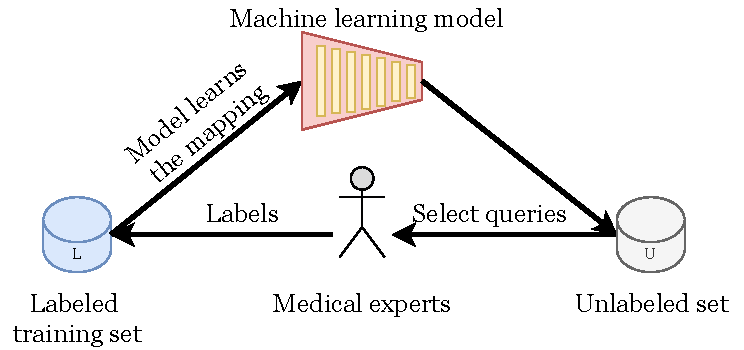
\includegraphics[width=0.75\textwidth]{figures/fig_active_learning.pdf}
\caption{The labeled set $\mathcal{L}$ is used to train the model. The trained model is then used to select data points, through an active learning algorithm, from the unlabeled set $\mathcal{U}$ for annotation. The selected data points are annotated by an expert and added to the labeled set $\mathcal{L}$.}
\label{fig:active_learning}
\end{figure}

% make this bigger and take help from https://link.springer.com/article/10.1007/s10994-019-05855-6
\section{Semi-supervised learning}
Semi-supervised learning (SSL)\cite{van2020} mitigates the requirement for labeled data by providing a means of leveraging unlabeled data. \\ Semi-supervised learning is a subfield of machine learning which tries to combine supervised learning with unsupervised learning. Semi-supervised learning algorithms, try to use the information available in the unlabeled data domain to help the performance of the model in the labeled data domain or vice versa. For instance, in case of a classification task, the data points without a label can be help with the classification task. For an unsupervised method such as clustering, it can be helpful to have some data points which are known to belong to a specific class. \\
There are many cases where unlabelled data can help in constructing a classifier. Consider the example of a regression model, where the model takes images of a house as input and it has to predict the price of a house. Suppose the model learns to predict a higher price for houses with a parking space compared to the houses which don't have this predictive property. This regression model might work well for the examples in the training set that contain the predictive property of having a parking space, but will fail when the input images do not contain that predictive property. For example, if a house doesn't have a parking space but it has other amenities such as a swimming pool, the model will still predict a lower price for that house. Semi-supervised learning can be helpful in this regard. Consider that the unlabeled dataset, might contain some data points which connect the predictive property of having a parking space to the property of containing a swimming pool. For instance, the property of having a parking space might co-occur with the property of having a balcony. Moreover, the property of having a balcony might co-occur with the property of having a swimming pool. Hence, the model might be able to predict a higher price for a house containing a swimming pool, even if it has not seen that property in the training set.\\
SSL operates on the assumption that the unlabeled data contains some prior information about the labeled data. Since unlabeled data can often be obtained with minimal human labor, any performance boost conferred by SSL often comes with low cost. \\

\begin{figure}[htbp]
\centering
\captionsetup{format=plain}
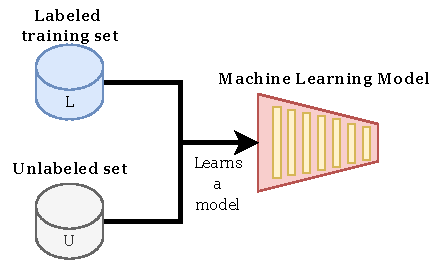
\includegraphics[width=0.5\textwidth]{figures/fig_semi_supervised_learning.pdf}
\caption{In SSL, both, the labeled set $\mathcal{L}$ and the unlabeled set $\mathcal{U}$, are used for learning a model. The information in the unlabeled set $\mathcal{U}$ is harnessed to improve the training performance on labeled set $\mathcal{L}$.}
\label{fig:semi_supervised_learning}
\end{figure}

\section{Annotation-efficient deep learning}
Deep learning methods are dependent upon large amounts of annotated data for their success \cite{sun2017}. In case of biomedical images, the annotations have to carried out by trained experts, so the process of annotations is time-consuming and expensive. Active learning algorithms try to minimize the need of annotations by selecting the data points which are most informative for annotation \cite{settles2009, sadafi2019, joshi2009}, but these algorithms are usually tested on real world image datasets e.g. ImageNet \cite{gal2016, ducoffe2015, holub2008}. However, biomedical images do not posses the same properties as real world images. Biomedical images have little variation between classes and posses little difference in color and textures \cite{matek2019, esteva2017}. Furthermore, biomedical image datasets have high class imbalance, which can have an significant impact on the results e.g. an algorithm which performs quite good for a dataset with no class imbalance might not perform as well for a dataset with high class imbalance. It has been shown that active learning can work well for biomedical image classification \cite{sadafi2019, smailagic2018} and segmentation \cite{yang2017}. However it is not clear that which active learning algorithm is more suited for a particular kind of biomedical image data and how can the active learning algorithms be combined with other deep learning methods for improving their performance. \\
It has been shown that pre-training methods such as transfer learning and self-supervised learning show great promise for initialization of network weights when low amount of annotation data is available \cite{chen2020, oord2018, newell2020, sagheer2019}. For transfer learning, the network weights are learned by training on a similar dataset and then reusing the learned weights for network initialization while training on the target dataset \cite{jing2020}. Initialization using pre-trained ImageNet weights is the most common transfer learning method and has been used in many biomedical applications for network initialization \cite{rajpurkar2017, wang2017}. However it is shown by Raghu and Zhang et al. \cite{raghu2019} that in transfer learning using ImageNet weights does not lead to an improvement in the performance for many biomedical image datasets. Moreover, it is shown that self-supervised learning on biomedical images can lead to an increase in performance \cite{holmberg2020}. \\
Finally, semi-supervised learning has been shown to increase the performance and stability of results \cite{sohn2020, tarvainen2017}. High-throughput methods are regularly employed in biomedical imaging \cite{blasi2016} to obtain a large number of unlabeled data points. However, as mentioned earlier, annotations are scarce in the domain of biomedical imaging. Thus, semi-supervised methods have great potential in this domain. \\
In this thesis, firstly, a comparison has been made between different active learning methods. Secondly, the performance of the active learning algorithm which performed the best, is further improved by adding pre-training and semi-supervised learning. To find out if a certain combination of the three active learning algorithms in addition to random sampling (baseline), three pre-training methods plus random initialization (baseline) and two training strategies which include supervised and semi-supervised learning, can outperform other conventional methods, an extensive grid search is performed and the results are gathered on three biomedical image datasets. As a result, an optimal strategy is found.